\chapter{SURF}

\section{Introduction}

SURF (Speeded Up Robust Features) est un descripteur tout comme son prédécesseur SIFT (Scale-Invariant Feature Transform). Son utilité réside dans le fait qu'il est capable de détecter des points d'intérêt sur une image pour ensuite pouvoir effectuer des tâches de reconstruction d'objet en 3D ou de reconnaissance d'objet, le sujet qui nous intéresse.

Son avantage par rapport à SIFT est qu'il est plusieurs fois plus rapides et ses créateurs affirment qu'il est en plus plus robuste aux transformations d'image. Utilisé pour son potentiel de reconnaissance d'objet, SURF nous permet d'extraire des features rapidement et facilement sur une image de caractère afin de pouvoir ensuite les classifier.

Afin de complémenter SURF, nous allons tenter d'utiliser un réseau de neurones pour la classification des caractères.

\section{Environnement}

SURF et le "bag of features" ont été exploités via MATLAB 2014b dans un environnement Windows 8.1 64bits. La gestion des fichiers s'est réalisée via git.

\section{Preprocessing}

Avant de pouvoir aisément travailler avec les images, il a été nécessaire de toutes les convertir en niveaux de gris, afin de ne travailler qu'avec une seule valeur. Un deuxième dataset avec les mêmes images redimensionnées vers le bas a aussi été créé.

\section{Extraction de features SURF}

De mon coté, j'ai suivi deux voies afin d'exploiter les possibilités de SURF. Tout d'abord en utilisant les features que l'on peut extraire via les descripteurs de SURF. En utilisant les méthodes fournies par Matlab (detectSURFFeatures), il est possible d'extraire les points d'intérêt de l'image (example en figure \ref{fig:surffeaturesexample}).

\begin{figure}[h]
\centering
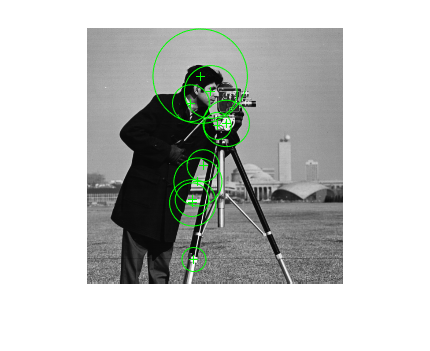
\includegraphics{pictures/DetectSURFFeaturesExample_01.png}
\caption{Points d'intérêt SURF}
\label{fig:surffeaturesexample}
\end{figure}

Après avoir récupéré les points, il est possible d'en extraire les features. Ces features vont dans le cas standard se traduire par un vecteur de taille 64 (un vecteur par point d'intérêt). Ceci est réalisé grâce à la méthode "extractFeatures". Cela va donc créer une matrice qui aura autant de lignes qu'il y a de points et 64 colonnes.

Avant de se lancer dans la classification, il sera néanmoins nécessaire de retravailler un peu ces features, car il n'est pas possible de générer une matrice pour notre réseau de neurones alors que les features sont elle-même déjà des matrices.

Une solution simple est d'aplatir simplement ces matrices de features, ainsi chaque point n'est qu'un morceau du vecteur qui va représenter l'image.

Un autre problème qui se pose est que parfois, certaines images ne possèdent pas assez de points d'intéret par rapport au nombre que l'on spécifie. Une solution a été de simplement ajouter des vecteurs vides afin de palier au manque de lignes de la matrice des features de l'image (qui sera convertie en vecteur je le rappelle).

\section{Classification}

\section{Résultats}

\section{Bag of features}

\section{Résultats}